% BDC223 Lecture 6: Light. Summary slides with TikZ figures.
% Build: see build.sh (lualatex, then one PNG per slide into ../../images/L06_light/).
% Curves drawn from equations are exact; panels marked "schematic" are illustrative only.
\documentclass[aspectratio=169,11pt]{beamer}
\usepackage[sfdefault,lining]{FiraSans}
\usepackage{amsmath}
\usefonttheme{professionalfonts}
\usepackage{firamath-otf}
\setmathrm{Fira Sans}
\usepackage{tikz}
\usepackage{pgfplots}
\pgfplotsset{compat=1.18,every axis/.append style={width=7.1cm}}
% Planck curve for a 5,778 K black body, normalised to 1 at 500 nm (hc/k = 1.4388e7 nm K)
\pgfmathdeclarefunction{bb}{1}{\pgfmathparse{(500/#1)^5/(exp(2489/#1)-1)*(exp(2489/500)-1)}}
\usetikzlibrary{arrows.meta,calc,decorations.pathmorphing,shapes.geometric,positioning}

% ---- look -------------------------------------------------------------
\definecolor{ink}{HTML}{1F2A37}
\definecolor{accent}{HTML}{0F766E}
\definecolor{soft}{HTML}{E6F2F1}
\definecolor{sea}{HTML}{1D4E89}
\definecolor{grey}{HTML}{6B7280}
\setbeamercolor{frametitle}{fg=white,bg=ink}
\setbeamercolor{normal text}{fg=ink,bg=white}
\setbeamercolor{itemize item}{fg=accent}
\setbeamercolor{itemize subitem}{fg=accent}
\setbeamertemplate{itemize item}{\small$\blacktriangleright$}
\setbeamertemplate{itemize subitem}{\footnotesize\textendash}
\setbeamertemplate{navigation symbols}{}
\setbeamerfont{frametitle}{size=\Large,series=\bfseries}
\setbeamertemplate{frametitle}{%
  \nointerlineskip
  \begin{beamercolorbox}[wd=\paperwidth,ht=2.4em,dp=0.9em,leftskip=1.2em]{frametitle}
    \insertframetitle
  \end{beamercolorbox}}
\setbeamertemplate{footline}{%
  \hbox to \paperwidth{\hspace{1.2em}\color{grey}\tiny BDC223 Plant Ecophysiology \textbar{} Lecture 6: Light\hfill\insertframenumber\hspace{1.2em}}\vspace{0.6em}}
\setlength{\leftmargini}{1.4em}
% wavelength (nm) to an RGB colour that pgf can use
\newcommand{\wavecol}[2]{\definecolor{tmpwave}{wave}{#2}\colorlet{#1}[rgb]{tmpwave}}
\newcommand{\schematic}{\par\vspace{2pt}{\color{grey}\scriptsize Schematic; not to scale.}}
\newcommand{\twocol}[2]{%
  \begin{columns}[c,onlytextwidth]
    \begin{column}{0.47\textwidth}#1\end{column}
    \begin{column}{0.50\textwidth}\centering #2\end{column}
  \end{columns}}

\begin{document}

% 1 ---------------------------------------------------------------------
\begin{frame}{Light: a resource, a signal and a stress}
\twocol{
\begin{itemize}
  \item Light is the energy source for photosynthesis
  \item It is also a signal for timing development
  \item In excess, it damages the photosynthetic apparatus
  \item Atmosphere, canopies and water change light before it reaches a leaf or alga
\end{itemize}}{
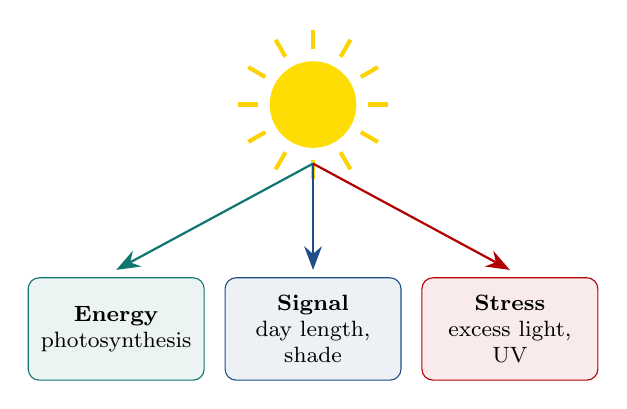
\begin{tikzpicture}[font=\small]
  \fill[yellow!80!orange] (0,3.2) circle (0.55);
  \foreach \a in {0,30,...,330} \draw[yellow!70!orange,line width=1.5pt] ($(0,3.2)+(\a:0.7)$) -- ($(0,3.2)+(\a:0.95)$);
  \foreach \x/\lab/\col in {-2.5/{\textbf{Energy}\\photosynthesis}/accent, 0/{\textbf{Signal}\\day length,\\shade}/sea, 2.5/{\textbf{Stress}\\excess light,\\UV}/red!70!black}{
    \draw[-{Stealth[length=3mm]},thick,\col] (0,2.45) -- (\x,1.1);
    \node[draw=\col,fill=\col!8,rounded corners,align=center,text width=2.0cm,minimum height=1.3cm,font=\footnotesize] at (\x,0.35) {\lab};}
\end{tikzpicture}}
\end{frame}

% 2 ---------------------------------------------------------------------
\begin{frame}{Why light matters to plants}
\twocol{
\begin{itemize}
  \item \textbf{Energy}: photosynthesis converts light energy to chemical energy
  \item \textbf{Signal}:
  \begin{itemize}
    \item photoperiodism: response to day length (e.g.\ flowering)
    \item circadian rhythms: internal clocks kept in time by light
    \item photomorphogenesis: light controls growth and form
  \end{itemize}
  \item \textbf{Stress}: too much light or UV damages photosystems
  \item With temperature, light largely sets where plants grow
\end{itemize}}{
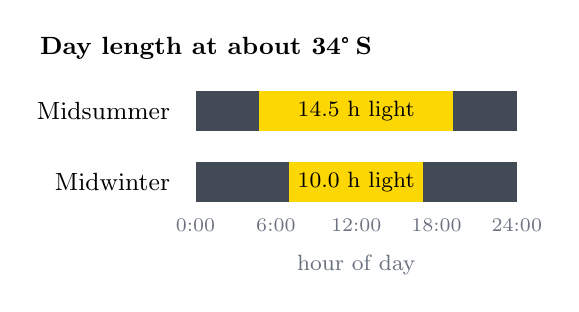
\begin{tikzpicture}[font=\small]
  % day length bars
  \node[anchor=west] at (-0.2,3.0) {\textbf{Day length at about 34\textdegree\,S}};
  \foreach \y/\lab/\h in {2.2/Midsummer/14.5, 1.3/Midwinter/10.0}{
    \node[anchor=east] at (1.7,\y) {\lab};
    \fill[ink!85] (1.9,\y-0.25) rectangle (1.9+24*0.17,\y+0.25);
    \fill[yellow!75!orange] ({1.9+(12-\h/2)*0.17},\y-0.25) rectangle ({1.9+(12+\h/2)*0.17},\y+0.25);
    \node[font=\footnotesize] at ({1.9+12*0.17},\y) {\h\ h light};}
  \foreach \t in {0,6,12,18,24} \node[font=\scriptsize,grey] at ({1.9+\t*0.17},0.75) {\t:00};
  \node[font=\footnotesize,grey,align=center] at ({1.9+12*0.17},0.25) {hour of day};
\end{tikzpicture}}
\end{frame}

% 3 ---------------------------------------------------------------------
\begin{frame}{Light varies in space and time}
\twocol{
\begin{itemize}
  \item \textbf{Predictable}: day length and Sun height change with latitude and season
  \item \textbf{Unpredictable}: cloud, aerosols, moving leaves, waves
  \item Annual totals vary little between years
  \item Minutes to days: light varies a great deal
  \item \textbf{PPFD} (photosynthetic photon flux density): photons of 400--700 nm per m$^2$ per s, in $\mu$mol m$^{-2}$ s$^{-1}$
\end{itemize}}{
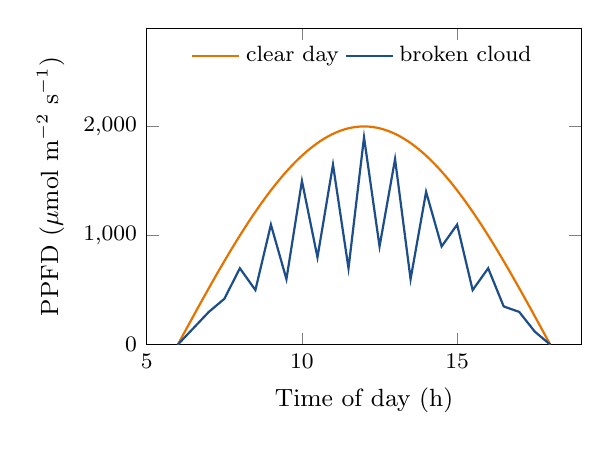
\begin{tikzpicture}
\begin{axis}[height=5.6cm,xmin=5,xmax=19,ymin=0,ymax=2900,
  xlabel={Time of day (h)},ylabel={PPFD ($\mu$mol m$^{-2}$ s$^{-1}$)},
  tick label style={font=\footnotesize},label style={font=\small},
  legend columns=2,legend style={font=\footnotesize,draw=none,fill=none,at={(0.5,0.98)},anchor=north}]
  \addplot[domain=6:18,samples=100,thick,orange!90!black] {2000*sin(deg(pi*(x-6)/12))};
  \addlegendentry{clear day}
  \addplot[thick,sea,mark=none] coordinates {(6,0)(7,300)(7.5,420)(8,700)(8.5,500)(9,1100)(9.5,600)(10,1500)(10.5,800)(11,1650)
     (11.5,700)(12,1900)(12.5,900)(13,1700)(13.5,600)(14,1400)(14.5,900)(15,1100)(15.5,500)(16,700)(16.5,350)(17,300)(17.5,120)(18,0)};
  \addlegendentry{broken cloud}
\end{axis}
\end{tikzpicture}
\schematic}
\end{frame}

% 4 ---------------------------------------------------------------------
\begin{frame}{Light quantity and light quality}
\twocol{
\begin{itemize}
  \item \textbf{Quantity}: how much light, regardless of colour
  \item \textbf{Quality}: spectral composition, i.e.\ the relative amounts of each wavelength
  \item Quality includes UV and far-red, which we cannot see
  \item Quantity and quality vary independently
\end{itemize}}{
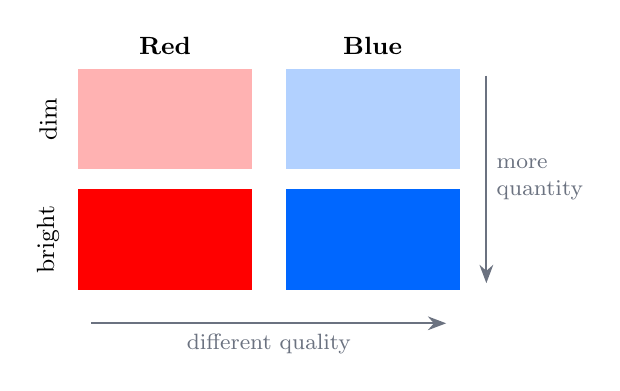
\begin{tikzpicture}[font=\small,scale=0.85]
  \wavecol{r}{650}\wavecol{b}{460}
  \foreach \c/\x/\lab in {r/0/Red, b/3.1/Blue}{
    \fill[\c!30] (\x,2.1) rectangle (\x+2.6,3.6);
    \fill[\c] (\x,0.3) rectangle (\x+2.6,1.8);
    \node at (\x+1.3,3.95) {\textbf{\lab}};}
  \node[rotate=90] at (-0.45,2.85) {dim};
  \node[rotate=90] at (-0.45,1.05) {bright};
  \draw[-{Stealth},thick,grey] (6.1,3.5) -- node[right,align=left,font=\footnotesize]{more\\quantity} (6.1,0.4);
  \draw[-{Stealth},thick,grey] (0.2,-0.2) -- node[below,font=\footnotesize]{different quality} (5.5,-0.2);
\end{tikzpicture}}
\end{frame}

% 5 ---------------------------------------------------------------------
\begin{frame}{The electromagnetic spectrum}
\begin{itemize}
  \item Visible light is a narrow band, about 390--750 nm for the human eye
  \item Plants use a similar band for photosynthesis (PAR, 400--700 nm)
  \item UV lies at shorter wavelengths, infrared at longer wavelengths
\end{itemize}
\vspace{4pt}
\centering
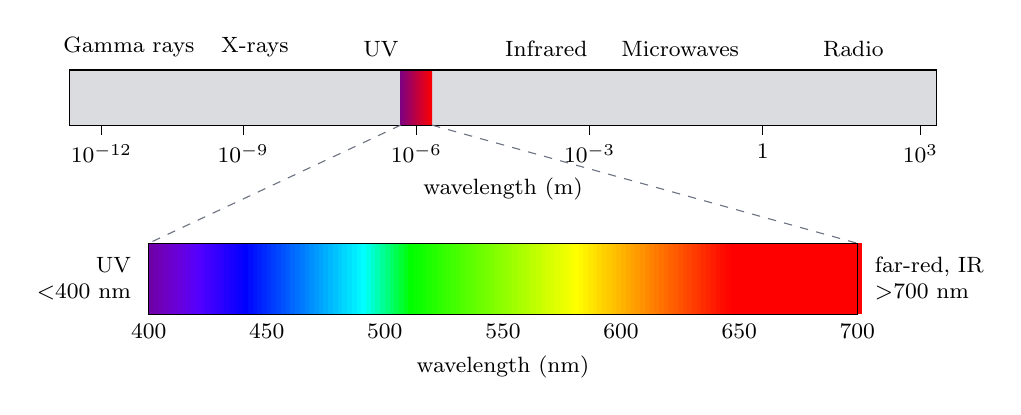
\begin{tikzpicture}[font=\footnotesize]
  % log-scale band (metres)
  \foreach \x/\lab in {0/Gamma rays,1.6/X-rays,3.2/UV,4.25/,5.3/Infrared,7.0/Microwaves,9.2/Radio}{\node[anchor=south] at (\x+0.75,0.75) {\lab};}
  \fill[grey!25] (0,0) rectangle (4.2,0.7);
  \fill[grey!25] (4.6,0) rectangle (11,0.7);
  \shade[left color=violet,right color=red] (4.2,0) rectangle (4.6,0.7);
  \draw (0,0) rectangle (11,0.7);
  \foreach \x/\lab in {0.4/$10^{-12}$,2.2/$10^{-9}$,4.4/$10^{-6}$,6.6/$10^{-3}$,8.8/$1$,10.8/$10^{3}$}{
     \draw (\x,0) -- (\x,-0.12); \node[below] at (\x,-0.12) {\lab};}
  \node[below] at (5.5,-0.55) {wavelength (m)};
  % zoom
  \draw[dashed,grey] (4.2,0) -- (1.0,-1.5); \draw[dashed,grey] (4.6,0) -- (10.0,-1.5);
  \foreach \w in {400,402,...,700}{
     \wavecol{wc}{\w}
     \fill[wc] ({1.0+(\w-400)/300*9.0},-2.4) rectangle ({1.0+(\w-398)/300*9.0},-1.5);}
  \draw (1.0,-2.4) rectangle (10.0,-1.5);
  \foreach \w in {400,450,500,550,600,650,700}{\node[below] at ({1.0+(\w-400)/300*9.0},-2.4) {\w};}
  \node[below] at (5.5,-2.8) {wavelength (nm)};
  \node[anchor=east,align=right] at (0.9,-1.95) {UV\\$<$400 nm};
  \node[anchor=west,align=left] at (10.1,-1.95) {far-red, IR\\$>$700 nm};
\end{tikzpicture}
\end{frame}

% 6 ---------------------------------------------------------------------
\begin{frame}{Wavelength, frequency and photon energy}
\twocol{
\begin{itemize}
  \item $c = \lambda\nu$: short wavelength means high frequency
  \item Photon energy: $E = h\nu = hc/\lambda$
  \item Each blue photon carries more energy than each red photon
  \item This is per photon; total energy also depends on photon numbers
  \item 450 nm: 266 kJ mol$^{-1}$; 680 nm: 176 kJ mol$^{-1}$
\end{itemize}}{
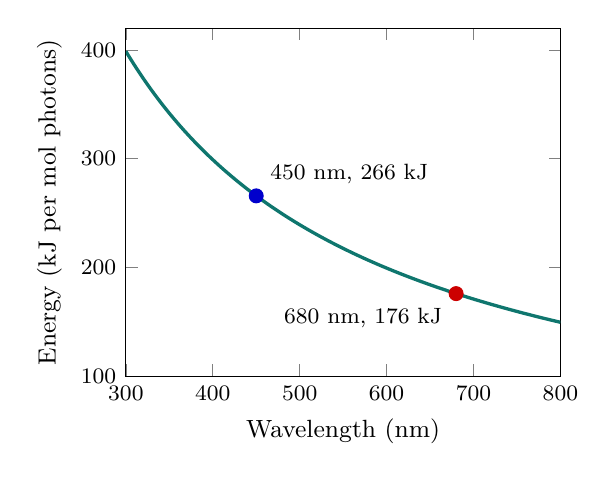
\begin{tikzpicture}
\begin{axis}[height=6cm,xmin=300,xmax=800,ymin=100,ymax=420,
  xlabel={Wavelength (nm)},ylabel={Energy (kJ per mol photons)},
  tick label style={font=\footnotesize},label style={font=\small}]
  \addplot[domain=300:800,samples=120,very thick,accent] {119627/x};
  \addplot[only marks,mark=*,mark size=2.5pt,blue!80!black] coordinates {(450,265.8)};
  \addplot[only marks,mark=*,mark size=2.5pt,red!80!black] coordinates {(680,175.9)};
  \node[anchor=south west,font=\footnotesize] at (axis cs:455,268) {450 nm, 266 kJ};
  \node[anchor=north east,font=\footnotesize] at (axis cs:675,172) {680 nm, 176 kJ};
\end{axis}
\end{tikzpicture}\\[-2pt]
{\color{grey}\scriptsize Curve: $E = N_A hc/\lambda$.}}
\end{frame}

% 7 ---------------------------------------------------------------------
\begin{frame}{Ultraviolet radiation}
\twocol{
\begin{itemize}
  \item UV-C 100--280 nm, UV-B 280--315 nm, UV-A 315--400 nm
  \item Ozone removes UV-C and most UV-B; ground UV starts at about 290--295 nm
  \item Not ionising, but UV-B damages DNA and photosystem II (D1 protein)
  \item Plants sense UV (UVR8; cryptochromes, phototropins) and respond with flavonoid sunscreens
\end{itemize}}{
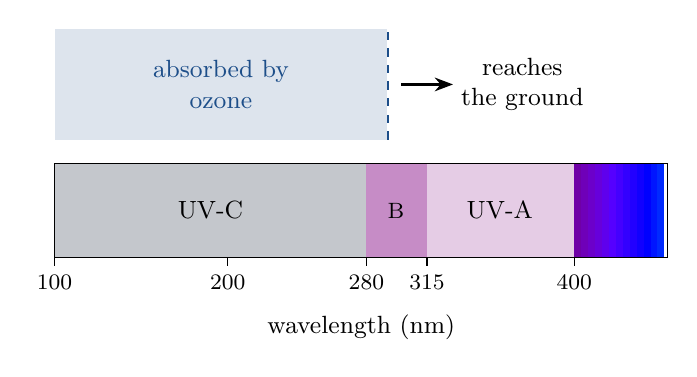
\begin{tikzpicture}[font=\small,x=0.022cm]
  \fill[grey!40] (100,0) rectangle (280,1.2);
  \fill[violet!45] (280,0) rectangle (315,1.2);
  \fill[violet!20] (315,0) rectangle (400,1.2);
  \foreach \w in {400,404,...,450}{\wavecol{wc}{\w}\fill[wc] (\w,0) rectangle (\w+4,1.2);}
  \draw (100,0) rectangle (454,1.2);
  \node at (190,0.6) {UV-C}; \node[font=\footnotesize] at (297,0.6) {B}; \node at (357,0.6) {UV-A};
  \foreach \w in {100,200,280,315,400}{\draw (\w,0)--(\w,-0.1); \node[below,font=\footnotesize] at (\w,-0.1) {\w};}
  \node[below] at (277,-0.6) {wavelength (nm)};
  % ozone filter
  \draw[very thick,sea,dashed] (292,1.5) -- (292,2.9);
  \fill[sea!15] (100,1.5) rectangle (292,2.9);
  \node[align=center,sea] at (196,2.2) {absorbed by\\ozone};
  \node[align=center] at (370,2.2) {reaches\\the ground};
  \draw[-{Stealth},thick] (300,2.2) -- (330,2.2);
\end{tikzpicture}}
\end{frame}

% 8 ---------------------------------------------------------------------
\begin{frame}{Infrared and far-red light}
\twocol{
\begin{itemize}
  \item About half of solar energy is infrared; beyond about 750 nm it acts mainly as heat
  \item Far-red (700--750 nm) is biologically active
  \item Phytochrome switches between a red-absorbing form (Pr, peak near 660 nm) and a far-red-absorbing form (Pfr, peak near 730 nm)
  \item Far-red adds to photosynthesis via photosystem I (Emerson enhancement)
\end{itemize}}{
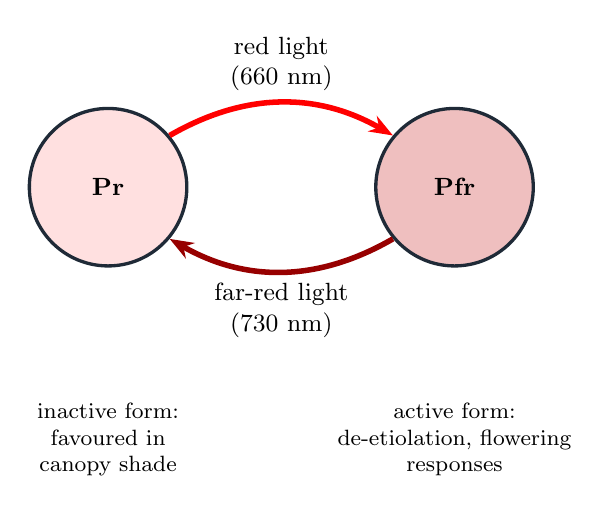
\begin{tikzpicture}[font=\small]
  \wavecol{rr}{660}\wavecol{fr}{730}
  \node[draw=ink,very thick,circle,minimum size=2cm,fill=rr!12] (pr) at (0,0) {\textbf{Pr}};
  \node[draw=ink,very thick,circle,minimum size=2cm,fill=fr!25] (pfr) at (4.4,0) {\textbf{Pfr}};
  \draw[-{Stealth[length=3mm]},line width=2pt,rr] (pr.40) to[bend left=30] node[above,black,align=center]{red light\\(660 nm)} (pfr.140);
  \draw[-{Stealth[length=3mm]},line width=2pt,fr!80!black] (pfr.220) to[bend left=30] node[below,black,align=center]{far-red light\\(730 nm)} (pr.320);
  \node[below=1.6cm of pfr,align=center,font=\footnotesize] {active form:\\de-etiolation, flowering\\responses};
  \node[below=1.6cm of pr,align=center,font=\footnotesize] {inactive form:\\favoured in\\canopy shade};
\end{tikzpicture}}
\end{frame}

% 9 ---------------------------------------------------------------------
\begin{frame}{Photosynthetically active radiation (PAR)}
\twocol{
\begin{itemize}
  \item \textbf{PAR = 400--700 nm} (McCree's definition)
  \item Quantum sensors measure this band
  \item The limits are a convention: some photons at 700--750 nm are also used (``extended PAR'')
  \item PAR is roughly 45--50\% of the energy in sunlight at the ground
\end{itemize}}{
\begin{tikzpicture}
\begin{axis}[height=5.8cm,xmin=280,xmax=1400,ymin=0,ymax=1.08,
  xlabel={Wavelength (nm)},ylabel={Relative spectral irradiance},yticklabels={},
  tick label style={font=\footnotesize},label style={font=\small},clip=false]
  \addplot[draw=none,fill=accent!25,domain=400:700,samples=60] {bb(x)/1.0} \closedcycle;
  \addplot[draw=none,fill=accent!10,domain=700:750,samples=10] {bb(x)} \closedcycle;
  \addplot[domain=280:1400,samples=150,thick,ink] {bb(x)};
  \node[font=\small,accent!70!black] at (axis cs:550,0.45) {\textbf{PAR}};
  \node[font=\scriptsize,accent!70!black,rotate=90] at (axis cs:725,0.35) {extended};
  \node[font=\footnotesize] at (axis cs:330,1.0) {UV};
  \node[font=\footnotesize] at (axis cs:1050,0.6) {infrared};
\end{axis}
\end{tikzpicture}\\[-2pt]
{\color{grey}\scriptsize Curve: 5,778 K black body, a schematic of sunlight without atmospheric absorption.}}
\end{frame}

% 10 --------------------------------------------------------------------
\begin{frame}{Photochemical equivalence}
\twocol{
\begin{itemize}
  \item One absorbed photon excites one electron, whatever its wavelength (Stark--Einstein law)
  \item Blue light: higher excited state, then a drop to the lowest one, losing heat
  \item Only the lowest excited state drives photochemistry
  \item So count photons: measure light in moles of photons
  \item Red photons are used slightly more efficiently than blue
\end{itemize}}{
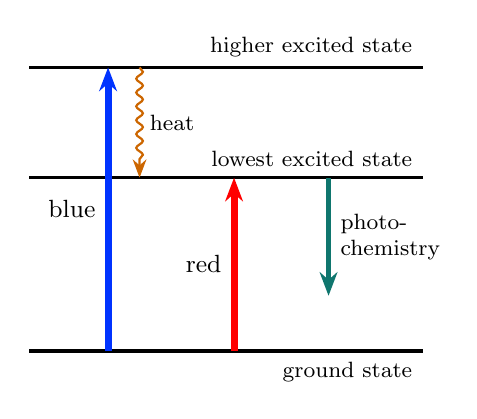
\begin{tikzpicture}[font=\small]
  \wavecol{bb}{450}\wavecol{rr}{680}
  \draw[very thick] (0,0) -- (5,0) node[below left,font=\footnotesize] {ground state};
  \draw[very thick] (0,2.2) -- (5,2.2) node[above left,font=\footnotesize] {lowest excited state};
  \draw[very thick] (0,3.6) -- (5,3.6) node[above left,font=\footnotesize] {higher excited state};
  \draw[-{Stealth[length=3mm]},line width=2.5pt,bb] (1,0) -- node[left,black]{blue} (1,3.6);
  \draw[-{Stealth[length=3mm]},line width=2.5pt,rr] (2.6,0) -- node[left,black]{red} (2.6,2.2);
  \draw[-{Stealth},thick,decorate,decoration={snake,amplitude=1.2pt,segment length=5pt,post length=2mm},orange!80!black] (1.4,3.6) -- node[right,black,font=\footnotesize]{heat} (1.4,2.2);
  \draw[-{Stealth[length=3mm]},line width=2pt,accent] (3.8,2.2) -- node[right,black,align=left,font=\footnotesize] {photo-\\chemistry} (3.8,0.7);
\end{tikzpicture}}
\end{frame}

% 11 --------------------------------------------------------------------
\begin{frame}{Light in the atmosphere}
\twocol{
\begin{itemize}
  \item Low Sun: light spread over more ground and a longer path through air
  \item Air molecules scatter blue strongly (Rayleigh), so the sky is blue
  \item Ozone absorbs UV-B; water vapour and CO$_2$ absorb parts of the IR
  \item Thick cloud can remove more than 80\% of light
  \item \textbf{Direct} light: a beam from the Sun's disc; \textbf{diffuse} light: scattered, from all directions
\end{itemize}}{
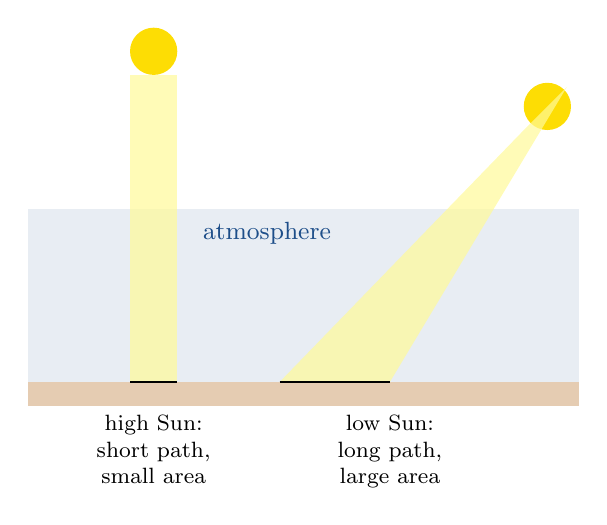
\begin{tikzpicture}[font=\small]
  \fill[sea!10] (0,0) rectangle (7,2.2);
  \node[sea,anchor=north west] at (2.1,2.15) {atmosphere};
  \fill[brown!40] (0,-0.3) rectangle (7,0);
  % high sun
  \fill[yellow!80!orange] (1.6,4.2) circle (0.3);
  \fill[yellow!40,opacity=0.7] (1.3,3.9) -- (1.9,3.9) -- (1.9,0) -- (1.3,0) -- cycle;
  \draw[thick] (1.3,0) -- (1.9,0);
  \node[below,font=\footnotesize,align=center] at (1.6,-0.3) {high Sun:\\short path,\\small area};
  % low sun
  \fill[yellow!80!orange] (6.6,3.5) circle (0.3);
  \fill[yellow!40,opacity=0.7] (6.35,3.25) -- (6.85,3.75) -- (4.6,0) -- (3.2,0) -- cycle;
  \draw[thick] (3.2,0) -- (4.6,0);
  \node[below,font=\footnotesize,align=center] at (4.6,-0.3) {low Sun:\\long path,\\large area};
\end{tikzpicture}}
\end{frame}

% 12 --------------------------------------------------------------------
\begin{frame}{Light under plant canopies}
\twocol{
\begin{itemize}
  \item Light declines exponentially with leaf area: $I = I_0\,e^{-k\cdot\text{LAI}}$
  \item LAI = leaf area per unit ground area; $k$ larger for horizontal leaves
  \item LAI = 4, $k = 0.6$: about 9\% of light reaches the ground
  \item Leaves absorb red but pass far-red: R:FR falls from about 1.2 to below 0.3
  \item Low R:FR triggers shade avoidance; sunflecks supply much forest-floor light
\end{itemize}}{
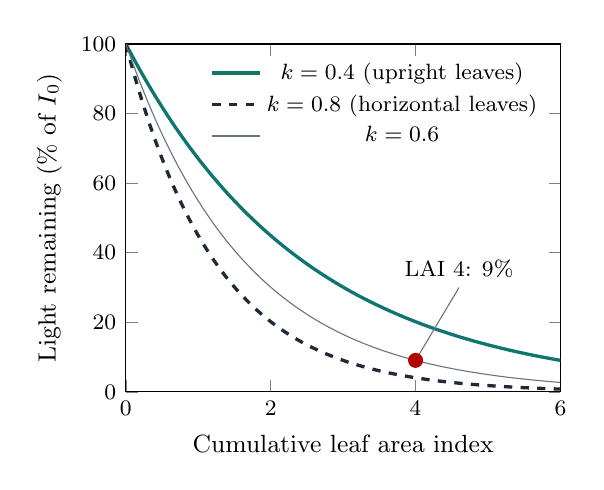
\begin{tikzpicture}
\begin{axis}[height=6cm,xmin=0,xmax=6,ymin=0,ymax=100,
  xlabel={Cumulative leaf area index},ylabel={Light remaining (\% of $I_0$)},
  tick label style={font=\footnotesize},label style={font=\small},
  legend style={font=\footnotesize,draw=none,fill=none}]
  \addplot[domain=0:6,samples=80,very thick,accent] {100*exp(-0.4*x)}; \addlegendentry{$k = 0.4$ (upright leaves)}
  \addplot[domain=0:6,samples=80,very thick,dashed,ink] {100*exp(-0.8*x)}; \addlegendentry{$k = 0.8$ (horizontal leaves)}
  \addplot[domain=0:6,samples=80,thin,grey] {100*exp(-0.6*x)}; \addlegendentry{$k = 0.6$}
  \addplot[only marks,mark=*,mark size=2.5pt,red!70!black] coordinates {(4,9.07)};
  \draw[grey] (axis cs:4,9.07) -- (axis cs:4.6,30);\node[anchor=south,font=\footnotesize] at (axis cs:4.6,30) {LAI 4: 9\%};
\end{axis}
\end{tikzpicture}\\[-2pt]
{\color{grey}\scriptsize Curves: $I/I_0 = e^{-k\cdot\text{LAI}}$.}}
\end{frame}

% 13 --------------------------------------------------------------------
\begin{frame}{Why red light disappears first in water}
\twocol{
\begin{itemize}
  \item Water molecules absorb red and IR strongly (bond vibrations), blue weakly
  \item At 700 nm, absorption is about 40--140 times that at 420--480 nm
  \item Red is gone within the top few metres; blue goes deepest in clear ocean
  \item The sea looks blue: red absorbed, blue scattered back by water
\end{itemize}}{
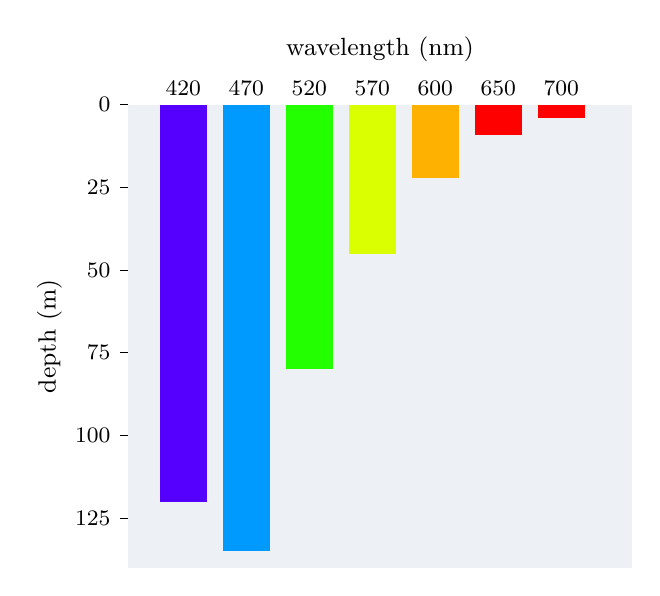
\begin{tikzpicture}[font=\small,y=-0.042cm]
  \fill[sea!8] (0,0) rectangle (6.4,140);
  \foreach \w/\d/\x in {420/120/0.4,470/135/1.2,520/80/2.0,570/45/2.8,600/22/3.6,650/9/4.4,700/4/5.2}{
     \wavecol{wc}{\w}
     \fill[wc] (\x,0) rectangle (\x+0.6,\d);
     \node[above,font=\footnotesize] at (\x+0.3,0) {\w};}
  \node[above=12pt] at (3.2,0) {wavelength (nm)};
  \foreach \z in {0,25,50,75,100,125}{\draw (0,\z) -- (-0.1,\z); \node[left,font=\footnotesize] at (-0.1,\z) {\z};}
  \node[rotate=90] at (-1.0,70) {depth (m)};
\end{tikzpicture}\\
{\color{grey}\scriptsize Schematic: approximate depth reached by each wavelength in clear ocean water.}}
\end{frame}

% 14 --------------------------------------------------------------------
\begin{frame}{The Beer--Lambert law in water}
\twocol{
\begin{itemize}
  \item $I_z = I_0\,e^{-K_d z}$; $K_d$ = diffuse attenuation coefficient (m$^{-1}$)
  \item From two depths: $K_d = \ln(I_1/I_2)/(z_2 - z_1)$
  \item Euphotic depth (1\% of surface PAR): $z_{eu} = \ln(100)/K_d \approx 4.6/K_d$
  \item Secchi disk estimate: $K_d \approx 1.7/z_{SD}$
  \item An approximation: $K_d$ differs between wavelengths and water layers
\end{itemize}}{
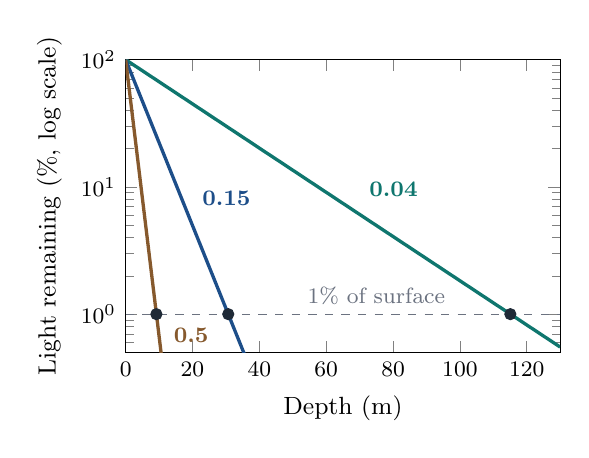
\begin{tikzpicture}
\begin{axis}[height=5.3cm,ymode=log,ymin=0.5,ymax=100,xmin=0,xmax=130,
  ylabel={Light remaining (\%, log scale)},xlabel={Depth (m)},
  tick label style={font=\footnotesize},label style={font=\small},
  ]
  \addplot[very thick,accent,domain=0:130,samples=60] {100*exp(-0.04*x)};
  \addplot[very thick,sea,domain=0:40,samples=40] {100*exp(-0.15*x)};
  \addplot[very thick,brown!70!black,domain=0:12,samples=30] {100*exp(-0.5*x)};
  \draw[dashed,grey] (axis cs:0,1) -- (axis cs:130,1);
  \node[font=\footnotesize,grey,anchor=south] at (axis cs:75,1) {1\% of surface};
  \addplot[only marks,mark=*,mark size=2pt,ink] coordinates {(9.2,1)(30.7,1)(115.1,1)};
        \node[anchor=west,font=\footnotesize\bfseries,brown!70!black] at (axis cs:11.5,0.68) {0.5};
  \node[anchor=south west,font=\footnotesize\bfseries,sea] at (axis cs:20,6) {0.15};
  \node[anchor=south west,font=\footnotesize\bfseries,accent] at (axis cs:70,7) {0.04};
\end{axis}
\end{tikzpicture}\\[-2pt]
{\color{grey}\scriptsize Curves: $I_z/I_0 = e^{-K_d z}$, labelled with $K_d$ (m$^{-1}$). Dots: euphotic depths (9, 31, 115 m).}}
\end{frame}

% 15 --------------------------------------------------------------------
\begin{frame}{Light zones in the ocean}
\twocol{
\begin{itemize}
  \item \textbf{Euphotic}: surface to 1\% PAR; nearly all marine photosynthesis; up to about 200 m in the clearest water, a few metres in turbid water
  \item \textbf{Dysphotic (twilight)}: to about 1,000 m; too little light for net photosynthesis
  \item \textbf{Aphotic}: below about 1,000 m; only bioluminescence
\end{itemize}}{
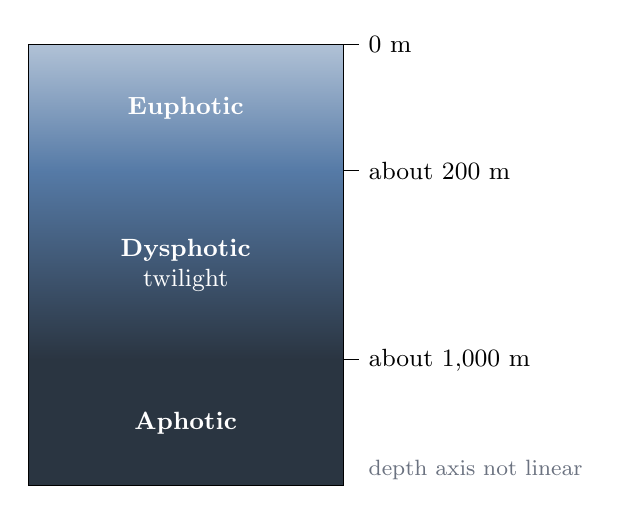
\begin{tikzpicture}[font=\small]
  \shade[top color=sea!35,bottom color=sea!75] (0,0) rectangle (4,-1.6);
  \shade[top color=sea!75,bottom color=ink!95] (0,-1.6) rectangle (4,-4.0);
  \fill[ink!95] (0,-4.0) rectangle (4,-5.6);
  \draw (0,0) rectangle (4,-5.6);
  \node[white,align=center] at (2,-0.8) {\textbf{Euphotic}};
  \node[white,align=center] at (2,-2.8) {\textbf{Dysphotic}\\twilight};
  \node[white,align=center] at (2,-4.8) {\textbf{Aphotic}};
  \foreach \y/\lab in {0/{0 m},-1.6/{about 200 m},-4.0/{about 1{,}000 m}}{\draw (4,\y) -- (4.2,\y); \node[right] at (4.2,\y) {\lab};}
  \node[right,grey,font=\footnotesize] at (4.2,-5.4) {depth axis not linear};
\end{tikzpicture}}
\end{frame}

% 16 --------------------------------------------------------------------
\begin{frame}{Heat from sunlight and the mixed layer}
\twocol{
\begin{itemize}
  \item Most solar heat is absorbed in the top metre or two (infrared and red)
  \item Wind and waves mix the heat down into the mixed layer
  \item Below it, temperature falls quickly through the thermocline
  \item Mixed-layer depth is set by mixing, not by light penetration
  \item South African west coast: upwelling brings cold deep water to the surface
\end{itemize}}{
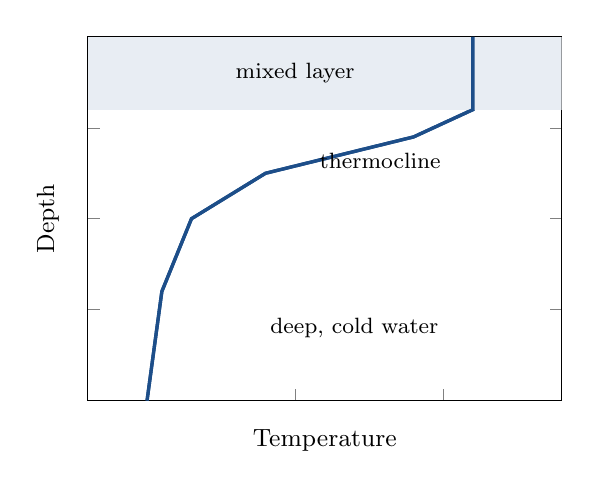
\begin{tikzpicture}
\begin{axis}[width=7.6cm,height=6.2cm,xmin=8,xmax=24,ymin=0,ymax=200,y dir=reverse,
  xlabel={Temperature},ylabel={Depth},xticklabels={},yticklabels={},
  label style={font=\small}]
  \addplot[very thick,sea] coordinates {(21,0)(21,40)(19,55)(14,75)(11.5,100)(10.5,140)(10,200)};
  \draw[fill=sea!10,draw=none] (axis cs:8,0) rectangle (axis cs:24,40);
  \addplot[very thick,sea] coordinates {(21,0)(21,40)(19,55)(14,75)(11.5,100)(10.5,140)(10,200)};
  \node[font=\footnotesize] at (axis cs:15,20) {mixed layer};
  \node[font=\footnotesize,anchor=west] at (axis cs:15.5,68) {thermocline};
  \node[font=\footnotesize] at (axis cs:17,160) {deep, cold water};
\end{axis}
\end{tikzpicture}
\schematic}
\end{frame}

% 17 --------------------------------------------------------------------
\begin{frame}{Coastal and open-ocean water}
\twocol{
\begin{itemize}
  \item Three groups of substances besides water attenuate light:
  \begin{itemize}
    \item phytoplankton pigments (absorb blue and red)
    \item coloured dissolved organic matter, CDOM (absorbs violet and blue)
    \item suspended particles, TSS (mainly scatter)
  \end{itemize}
  \item Coastal water: larger $K_d$, shallower euphotic zone
  \item Colour that penetrates furthest shifts from blue (ocean) to green, about 550 nm (coast)
\end{itemize}}{
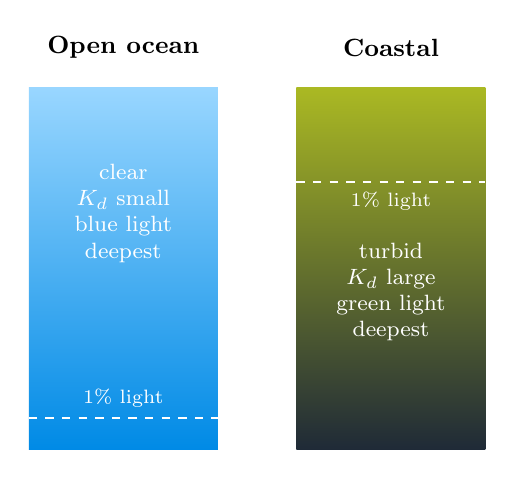
\begin{tikzpicture}[font=\small]
  \wavecol{deepb}{470}\wavecol{deepg}{550}
  \shade[top color=deepb!40,bottom color=deepb!90!black] (0,0) rectangle (2.4,-4.6);
  \shade[top color=deepg!45!brown,bottom color=ink] (3.4,0) rectangle (5.8,-4.6);
  \node[align=center] at (1.2,0.5) {\textbf{Open ocean}};
  \node[align=center] at (4.6,0.5) {\textbf{Coastal}};
  \node[white,align=center,font=\footnotesize] at (1.2,-1.6) {clear\\$K_d$ small\\blue light\\deepest};
  \node[white,align=center,font=\footnotesize] at (4.6,-2.6) {turbid\\$K_d$ large\\green light\\deepest};
  \draw[dashed,white,thick] (0,-4.2) -- (2.4,-4.2) node[midway,above,font=\scriptsize] {1\% light};
  \draw[dashed,white,thick] (3.4,-1.2) -- (5.8,-1.2) node[midway,below,font=\scriptsize] {1\% light};
\end{tikzpicture}
\schematic}
\end{frame}

% 18 --------------------------------------------------------------------
\begin{frame}{Measuring light: PPFD and the daily light integral}
\twocol{
\begin{itemize}
  \item PPFD: photons (400--700 nm) per m$^2$ per s, in $\mu$mol m$^{-2}$ s$^{-1}$
  \item $1\,\mu$mol m$^{-2}$ s$^{-1}$ = $6.022\times10^{17}$ photons m$^{-2}$ s$^{-1}$
  \item Summed over a day: daily light integral (DLI), mol m$^{-2}$ d$^{-1}$
  \item Mean 900 $\mu$mol m$^{-2}$ s$^{-1}$ for 12 h gives a DLI of 38.9 mol m$^{-2}$ d$^{-1}$
  \item A PPFD reading says nothing about light quality
\end{itemize}}{
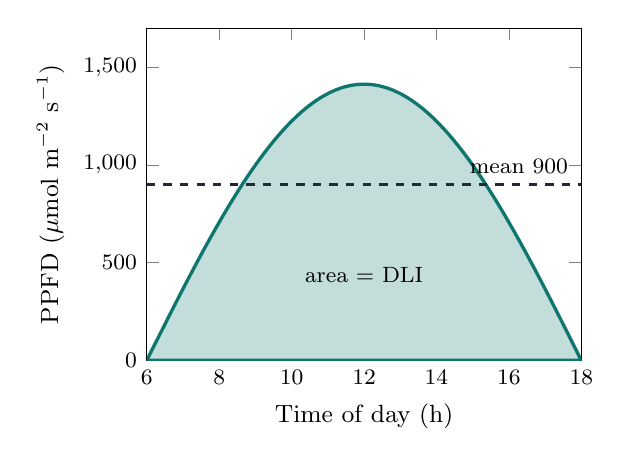
\begin{tikzpicture}
\begin{axis}[height=5.8cm,xmin=6,xmax=18,ymin=0,ymax=1700,
  xlabel={Time of day (h)},ylabel={PPFD ($\mu$mol m$^{-2}$ s$^{-1}$)},
  tick label style={font=\footnotesize},label style={font=\small}]
  \addplot[fill=accent!25,draw=accent,very thick,domain=6:18,samples=100] {1413.7*sin(deg(pi*(x-6)/12))} \closedcycle;
  \addplot[dashed,ink,thick] coordinates {(6,900)(18,900)};
  \node[font=\footnotesize,anchor=south] at (axis cs:12,350) {area = DLI};
  \node[font=\footnotesize,anchor=south east] at (axis cs:17.9,905) {mean 900};
\end{axis}
\end{tikzpicture}\\[-2pt]
{\color{grey}\scriptsize Idealised clear day: half-sine curve with a mean of 900 $\mu$mol m$^{-2}$ s$^{-1}$ over 12 h.}}
\end{frame}

% 19 --------------------------------------------------------------------
\begin{frame}{Typical light levels}
\twocol{
\begin{itemize}
  \item Clear-sky midday sun at sea level: about 2,000--2,300 $\mu$mol m$^{-2}$ s$^{-1}$
  \item Much lower in winter, early and late in the day, and under cloud
  \item Dense forest floor: may receive less than 2\% of the light above the canopy
  \item A well-lit office: about 5--10 $\mu$mol m$^{-2}$ s$^{-1}$
\end{itemize}}{
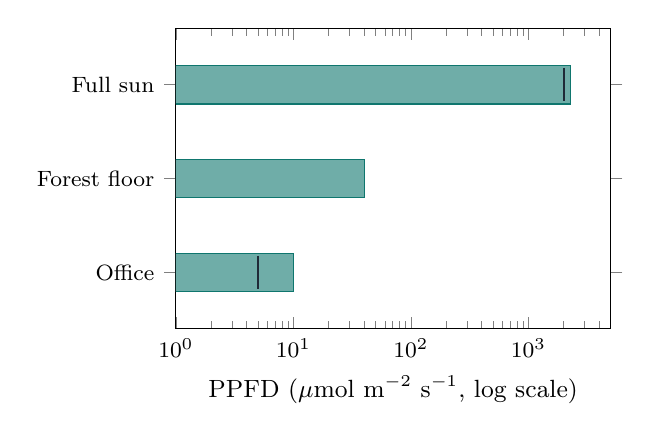
\begin{tikzpicture}
\begin{axis}[height=5.4cm,xbar,xmode=log,xmin=1,xmax=5000,
  ytick={1,2,3},yticklabels={{Office},{Forest floor},{Full sun}},ymin=0.4,ymax=3.6,
  xlabel={PPFD ($\mu$mol m$^{-2}$ s$^{-1}$, log scale)},bar width=14pt,
  tick label style={font=\footnotesize},label style={font=\small}]
  \addplot[fill=accent!60,draw=accent] coordinates {(10,1) (40,2) (2300,3)};
  \addplot[only marks,mark=|,mark size=6pt,ink,thick] coordinates {(5,1) (2000,3)};
\end{axis}
\end{tikzpicture}\\[-2pt]
{\color{grey}\scriptsize Bars show the upper value of each range; ticks the lower value. Forest floor: 2\% of 2,000.}}
\end{frame}

% 20 --------------------------------------------------------------------
\begin{frame}{Light sensors}
\twocol{
\begin{itemize}
  \item \textbf{Cosine-corrected (planar)}: flat collector; light from the whole upper hemisphere, weighted by the cosine of its angle from vertical (like a flat leaf)
  \item \textbf{Spherical (scalar)}: equal response from all directions (like a phytoplankton cell)
  \item \textbf{Spectroradiometer}: light at each wavelength (quality)
  \item \textbf{Pyranometer}: total solar energy, W m$^{-2}$
\end{itemize}}{
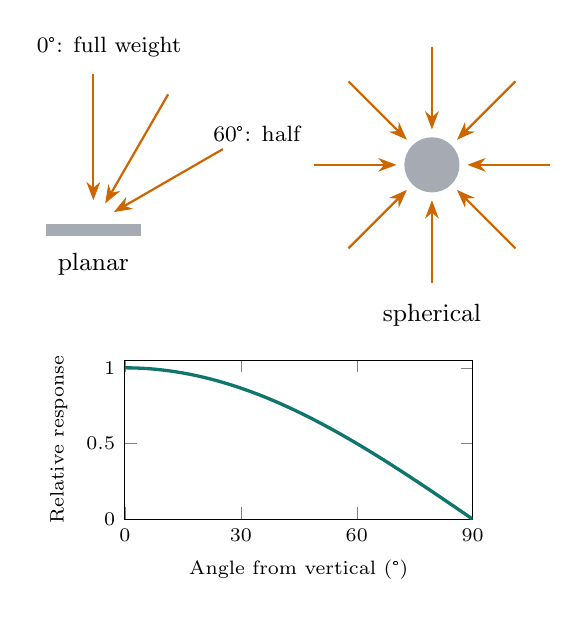
\begin{tikzpicture}[font=\small]
  % planar sensor
  \fill[grey!60] (-0.6,0) rectangle (0.6,0.15);
  \foreach \a in {90,60,30}{\draw[-{Stealth},thick,orange!80!black] ($(0,0.15)+(\a:1.9)$) -- ($(0,0.15)+(\a:0.3)$);}
  \node[font=\footnotesize] at (0.2,2.4) {0\textdegree: full weight};
  \node[font=\footnotesize,anchor=west] at (1.4,1.3) {60\textdegree: half};
  \node[below,align=center] at (0,-0.1) {planar};
  % spherical sensor
  \fill[grey!60] (4.3,0.9) circle (0.35);
  \foreach \a in {0,45,...,315}{\draw[-{Stealth},thick,orange!80!black] ($(4.3,0.9)+(\a:1.5)$) -- ($(4.3,0.9)+(\a:0.45)$);}
  \node[below,align=center] at (4.3,-0.75) {spherical};
  % cosine plot
  \begin{scope}[shift={(0.4,-3.6)}]
  \begin{axis}[width=6cm,height=3.6cm,xmin=0,xmax=90,ymin=0,ymax=1.05,xtick={0,30,60,90},
     xlabel={Angle from vertical (\textdegree)},ylabel={Relative response},
     tick label style={font=\scriptsize},label style={font=\scriptsize}]
     \addplot[very thick,accent,domain=0:90,samples=60] {cos(x)};
  \end{axis}
  \end{scope}
\end{tikzpicture}}
\end{frame}

% 21 --------------------------------------------------------------------
\begin{frame}{Three kinds of light units}
\twocol{
\begin{itemize}
  \item \textbf{Quantum} ($\mu$mol m$^{-2}$ s$^{-1}$): counts photons; the standard for photosynthesis
  \item \textbf{Radiometric} (W m$^{-2}$): energy; for energy balance and efficiency
  \item For sunlight: 1 W m$^{-2}$ PAR $\approx$ 4.57 $\mu$mol m$^{-2}$ s$^{-1}$ (depends on the spectrum)
  \item \textbf{Photometric} (lux, foot-candles): weighted by the human eye, peak at 555 nm; no exact conversion to PPFD
\end{itemize}}{
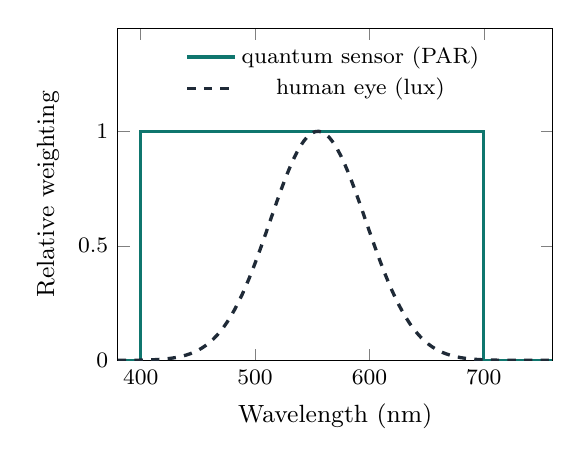
\begin{tikzpicture}
\begin{axis}[height=5.8cm,xmin=380,xmax=760,ymin=0,ymax=1.45,
  xlabel={Wavelength (nm)},ylabel={Relative weighting},
  tick label style={font=\footnotesize},label style={font=\small},
  legend style={font=\footnotesize,draw=none,fill=none,at={(0.5,0.98)},anchor=north}]
  \addplot[very thick,accent] coordinates {(380,0)(400,0)(400,1)(700,1)(700,0)(760,0)}; \addlegendentry{quantum sensor (PAR)}
  \addplot[very thick,dashed,ink,domain=380:760,samples=120] {exp(-0.5*((x-555)/42)^2)}; \addlegendentry{human eye (lux)}
\end{axis}
\end{tikzpicture}\\[-2pt]
{\color{grey}\scriptsize Schematic. Eye curve approximated by a Gaussian centred on 555 nm.}}
\end{frame}

% 22 --------------------------------------------------------------------
\begin{frame}{Summary: effects of each waveband}
\centering\small
\renewcommand{\arraystretch}{1.35}
\begin{tabular}{@{}p{2.1cm}p{2.4cm}p{8.6cm}@{}}
\textbf{Waveband} & \textbf{Wavelength} & \textbf{Main effects on plants}\\\hline
UV-B & 280--315 nm & Damages DNA and photosystem II; detected by UVR8; triggers flavonoid sunscreens\\
UV-A & 315--400 nm & Detected by cryptochromes and phototropins; little photosynthesis\\
PAR & 400--700 nm & Drives photosynthesis; blue sensed by cryptochromes and phototropins; red by phytochrome\\
Far-red & 700--750 nm & Detected by phytochrome (shade avoidance); aids photosynthesis via photosystem I\\
Infrared & $>$750 nm & Absorbed as heat; little photochemical effect\\\hline
\end{tabular}
\vspace{10pt}

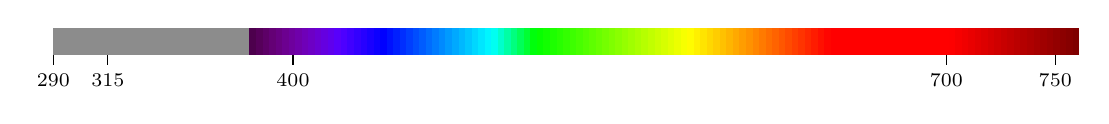
\begin{tikzpicture}
  \foreach \w in {290,293,...,760}{
    \ifnum\w<380 \definecolor{wc}{gray}{0.55}\else\wavecol{wc}{\w}\fi
    \fill[wc] ({(\w-290)/470*13},0) rectangle ({(\w-287)/470*13},0.35);}
  \foreach \w/\lab in {290/290,315/315,400/400,700/700,750/750}{\draw ({(\w-290)/470*13},0) -- ({(\w-290)/470*13},-0.12) node[below,font=\scriptsize]{\lab};}
\end{tikzpicture}
\end{frame}

\end{document}
